\documentclass[12pt]{article}
\usepackage[italian]{babel}
\usepackage{amsmath}
\usepackage{siunitx}
\usepackage{derivative}
\usepackage{graphicx}
\usepackage[a4paper, total={6in, 9in}]{geometry}
\usepackage{caption}
\usepackage{subcaption}
\usepackage{float}

\title{Sviluppo e caratterizzazione di un amplificatore RF per rivelatori criogenici}
\author{Nicolas Bigiotti}
\date{\today}


\begin{document}
\maketitle

Questa tesi si pone come obiettivo la realizzazione di un amplificatore RF e la successiva analisi qualitativa a bassa temperatura, amplificatori di questo tipo sono richiesti in molti ambiti sia di ricerca che industriali e la loro progettazione e caratterizzazione risulta essere diversa rispetto ad altri dispositivi operanti a frequenze più basse.

L'amplificatore è realizzato con transistor bipolari a eterogiunzione SiGe in configurazione a emettitore comune, la prima fase di progettazione ha riguardato la scelta del punto di lavoro, per garantire una bassa potenza dissipata dal transistor durante l'esercizio è stata scelta una corrente di collettore $I_{C}=\SI{8}{\milli\ampere}$ e una tensione collettore-emettitore $V_{CE}=\SI{3.0}{\volt}$, individuato il punto di lavoro è stato possibile dedicarsi alla progettazione della parte di segnale.

Un tipico amplificatore RF è composto da una rete di adattamento di ingresso con il compito di adattare l'impedenza del generatore a quella in ingresso del transistor, una di uscita per adattare l'uscita del transistor all'impedenza di carico e infine il transistor stesso, a differenza di quanto accade a bassa frequenza per studiare la risposta di piccolo segnale non viene utilizzato un modello a componenti concentrati del transistor ma si preferisce affidarsi a valori misurati e tabulati dei parametri di scattering.

Il primo passaggio di progettazione consiste nel valutare la stabilità della configurazione, non trattandosi di un amplificatore reazionato tutta la potenziale instabiltà è intrisecamente legata ai parametri di scattering del transistor che dipendono dalla frequenza di esercizio e dal punto di lavoro, in questo caso considerando un amplificatore a banda stretta centrata a $\SI{5}{\giga\hertz}$ il transistor risulta incodizionatamente stabile, vale a dire che indipendentemente dalle riflessioni introdotte dalle reti di adattamento l'amplificatore risulterà stabile e si ha piena libertà di progettazione di quest'ultime.

Garantita la stabilità si procede progettando le reti di adattamento in modo che venga garantito massimo guadagno alla frequenza di esercizio, per la realizzazione è stata utilizzata la tecnica a stub singolo che utilizza segmenti di linea di trasmissione opportunamente dimensionati per ottenere l'adattamento di impedenza voluto.
Una volta definito lo schema elettrico è stata realizzata la scheda con il software opensource KiCad in modo da rendere possibile la realizzazione del circuito stampato da una ditta specializzata, i componenti precedentemente selezionati e acquistati sono stati saldati sulla scheda.

Con l'ausilio di un analizzatore vettoriale di rete è stata fatta una misura completa dei parametri di scattering a temperatura ambiente, è stato possibile verificare la funzionalità dell'amplificatore osservando nel dominio del tempo e delle frequenze il segnale di uscita in presenza di una sinusoide in ingresso, le misure sono state ripetute a temperatura criogenica fino a $\SI{4}{\kelvin}$.
È stato realizzato anche un secondo amplificatore utilizzando componenti discreti per realizzare le reti di adattamento in modo da avere maggiore flessibilità in fase di misura, il percorso seguito per la progettazione è stato uguale al primo.
\begin{figure}[H]
    \centering
    \begin{subfigure}[b]{0.45\textwidth}
        \centering
        \includegraphics[scale=0.062]{img/IMG_2169.jpg}
        \caption{La scheda completa dopo la saldatura e il montaggio nell'involucro metallico necessario per un buon contatto termico con il criostato}
    \end{subfigure}
    \hfill
    \begin{subfigure}[b]{0.45\textwidth}
        \centering
        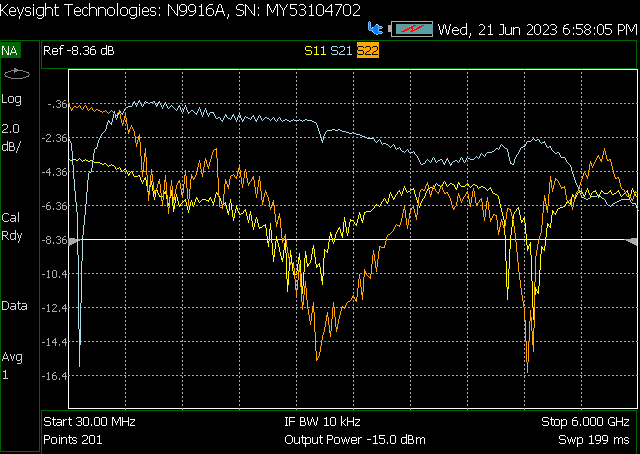
\includegraphics[scale=0.3]{img/STUB_NO_COP.png}
        \caption{Parametri di scattering $S_{11}$, $S_{22}$ e $S_{21}$ misurati a temperatura ambiente}
    \end{subfigure}
\end{figure}



\end{document}